\documentclass{ti2}

% Dateikodierung ist utf8
\usepackage[utf8]{inputenc}   
\usepackage{graphicx}
\usepackage{listings}
\usepackage{rotating}
\usepackage{nonfloat}
\lstset{
  numbers=left,
  numberstyle=\tiny,
  breaklines=true  
}

\begin{document}

% Nr, Abgabedatum, Gruppenleiter, Gruppenname, Name1...Name4
\Abgabeblatt{4}{28.11.2016}{Marc/Bingbin}{C05}%
                {Tabea Eggers}{Jan Fiedler}%
                {Florian Pflüger}{Jonas Schmutte}%

%\begin{listing}{1}
%\begin{listingcont}

\section*{Aufgabe 1}
Erstmal haben wir den Signalhandler geschrieben, da wir auf dem letzten Blatt bereits einen geschrieben haben, bot sich dies an.\\
Bevor wir uns an die Ausf"uhrung der Prozesse machten, haben wir die Methode "'findPathToCommand"' geschrieben, damit wir die richtigen Pfade bekommen.\\
Als dies richtig funktionierte, haben wir den Ausf"uhrungsteil geschrieben.\\
Danach haben wir diesen getestet und als funktionierend befunden.\\
Allerdings benutzen wir weder "'wait()"' noch "'waitpid()"', da wir mit dem Befehl "pause()", die richtige Funktionalit"at erzielten und mit den anderen beiden genannten, mehrere Bugs vorhanden waren.\\




\lstinputlisting[firstline=1,firstnumber=1,lastline=125]{aufgabe01/ti2sh.cc}
\subsection*{Tests}

F"uhrt die Beispielabfragen aus den Tutoriumsfolien aus.\\
Alle werden wie erwartet umgesetzt\\

\begin{minipage}{\linewidth}
	\centering%
	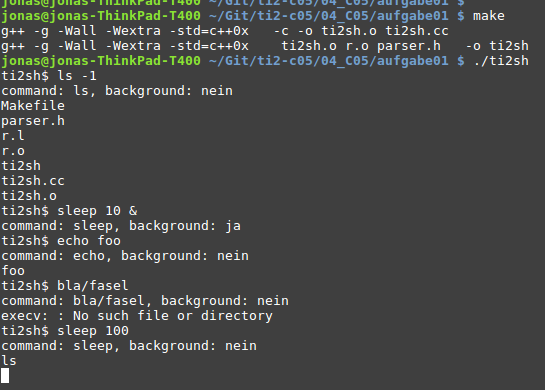
\includegraphics[width=\textwidth]{aufgabe01/test1.png}
\end{minipage}

W"ahrend des "'sleep 100" wird ls eingegeben, wie man sieht wird dieser erstmal nicht verarbeitet.\\
Nach ablaufen des sleeps wird der eben eingegebene ls-Befehl richtig verarbeitet.\\
\begin{minipage}{\linewidth}
	\centering%
	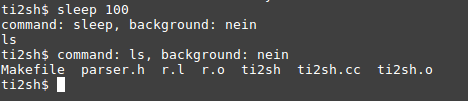
\includegraphics[width=\textwidth]{aufgabe01/test2.png}
\end{minipage}

Hier wird nochmal ls erst im Hintergrund und dann im Vordergrund ausgef"uhrt, man sieht deutlich, dass dies richtig funktioniert.\\

\begin{minipage}{\linewidth}
	\centering%
	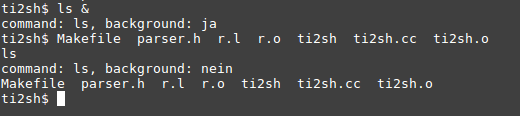
\includegraphics[width=\textwidth]{aufgabe01/test3.png}
\end{minipage}

Hier wird getestet, ob ein Befehl auch mit mehreren Optionen ausgef"uhrt werden kann, auch dies funktioniert.\\

\begin{minipage}{\linewidth}
	\centering%
	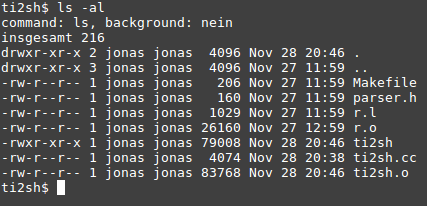
\includegraphics[width=\textwidth]{aufgabe01/test4.png}
\end{minipage}

Hier wird getest, ob absolute Pfadangaben richtig funktionieren, auch dies ist der Fall.\\
\begin{minipage}{\linewidth}
	\centering%
	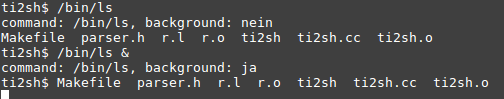
\includegraphics[width=\textwidth]{aufgabe01/test5.png}
\end{minipage}


\section*{Aufgabe 2}
zu a)\\
Einfügen der Anforderungen: \\\\
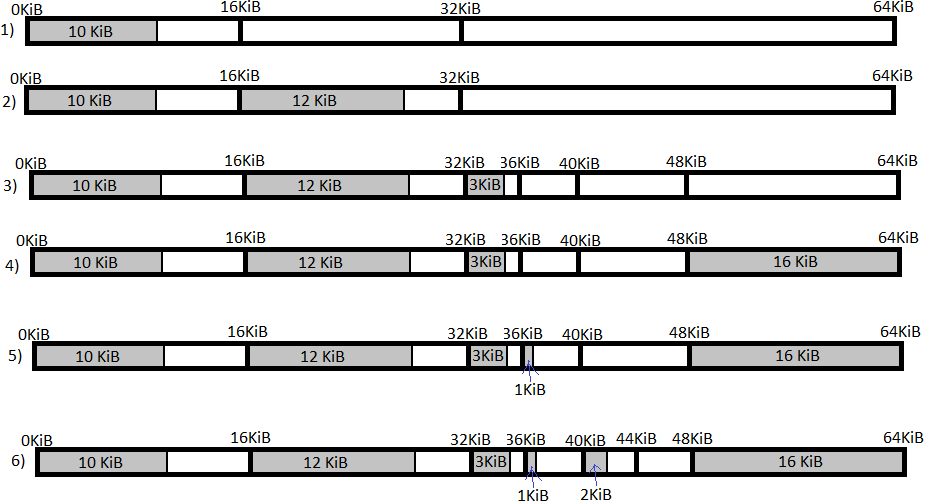
\includegraphics[width=1.05\textwidth]{Aufgabe2.png}
Anforderung für 20 KiB ist nicht erfüllbar, da kein Platz groß genug ist (siehe von Schritt 5) auf 6)). Deshalb wird in Schritt 6 auch die Anforderung von 2 KiB erfüllt (dafür ist genug Platz). Somit bleiben 6 freie Blöcke übrig: \\\\
\begin{tabular}[c]{|c|c|c|c|}
	\hline
	Block & Anfangsadresse & Endadresse & Größe \\
	\hline
	\hline
	1 & 10 KiB & 16 KiB & 6 KiB \\
	\hline
	2 & 28 KiB & 32 KiB & 4 KiB \\
	\hline
	3 & 35 KiB & 36 KiB & 1 KiB \\
	\hline
	4 & 37 KiB & 40 KiB & 3 KiB \\
	\hline
	5 & 42 KiB & 44 KiB & 2 KiB \\
	\hline
	6 & 44 KiB & 48 KiB & 4 KiB \\
	\hline
\end{tabular}\\\\
zu b)\\
Es gibt nun noch folgende Blöcke: \\\\
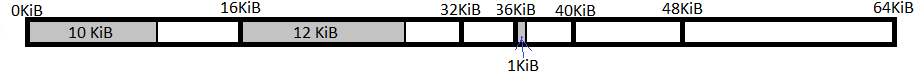
\includegraphics[width=1.05\textwidth]{Aufgabe2b.png} 
Nach der Freigabe kann keine Anforderung von 21 KiB erfüllt werden, da kein Speicherplatz groß genug ist. Wenn nun noch die Anforderung von 1 KiB freigegeben werden würde, würde die Anforderung von 21 KiB erfüllt werden können.

\section*{Aufgabe 3}
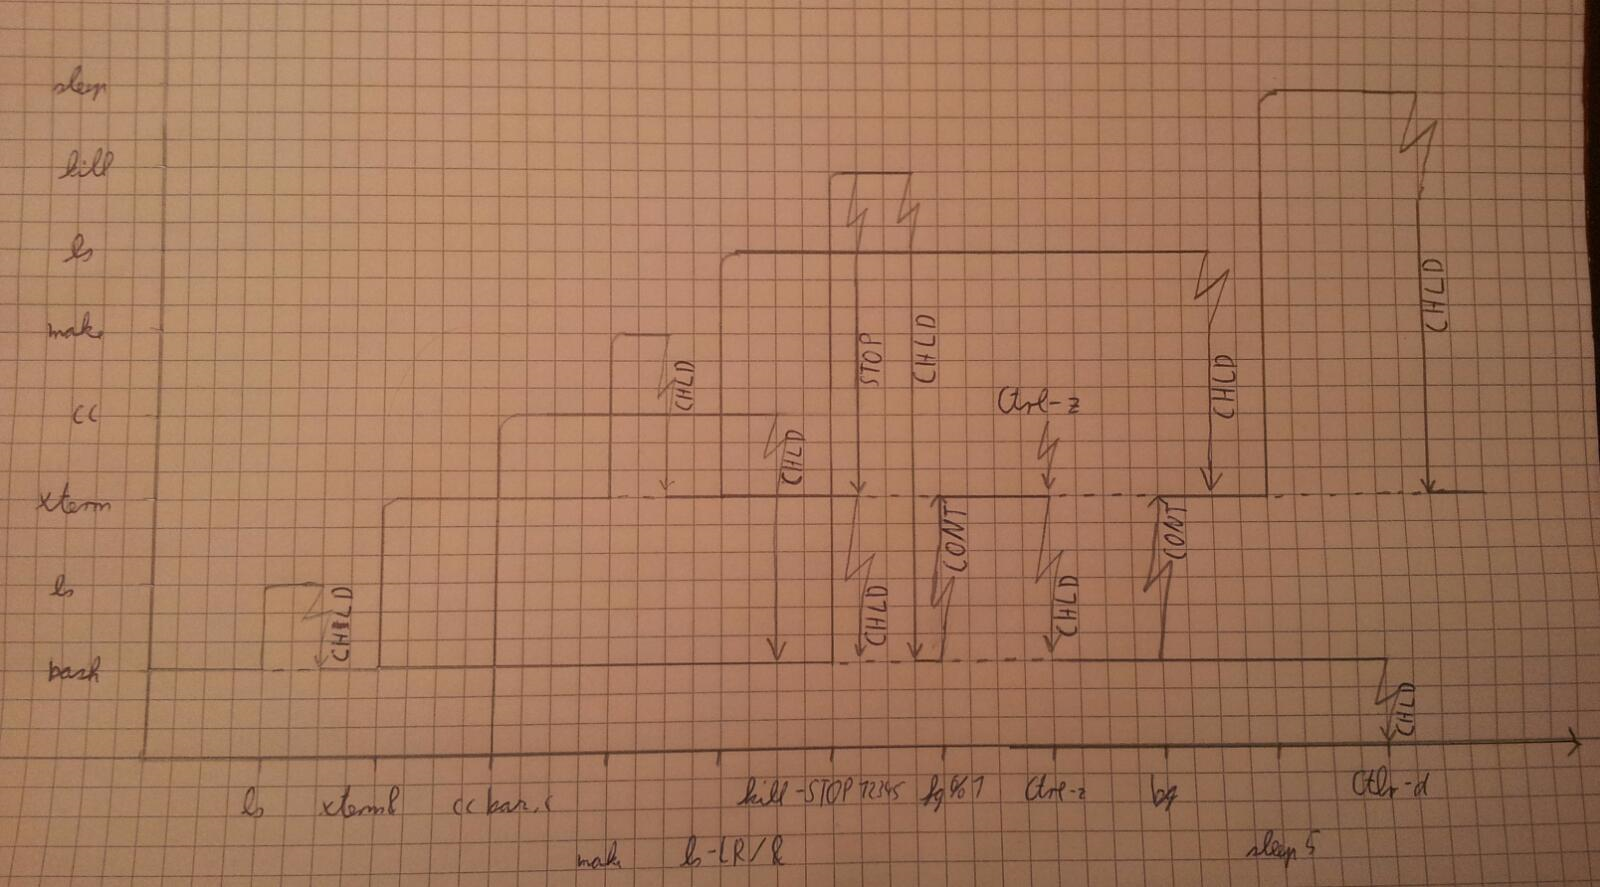
\includegraphics[width=\textwidth]{aufgabe3}

Die x-Achse stellt die Befehle dar, die y-Achse die Prozesse. Prozesse mit einem \&, die im Hintergrund laufen und irgendwann fertig sind, senden, beim Beenden, bei uns ein CHLD an ihren Vater, falls der beendet worden wäre, würde es an dessen Vater gesendet werden.\\
Am Ende gehört das in Schritt 2 gestartete Terminal zum Vater-Prozess der Bash aus Schritt 0, da diese an diesen vererbt wird, wenn die Bash beendet wird.

\end{document}
